\section{Iterative Pruning of Attention Heads}
\label{sec:pruning}

% \gn{I think rather than ``Attention Pruning for Model Compression'' or something?}\paul{Not sure I understand this comment}\gn{Sorry, what I meant was that it wasn't clear why this section was ``Heuristic Pruning of Attention Heads,'' as this also seemed to apply to the previous section as well. I changed the title to ``Iterative Pruning of Attention Heads.'' Does that seem OK? It seems more descriptive perhaps.}

% The results from Section \ref{sec:are_all_heads_important} raise a natural question: do we even need more than one head at test time?

In our ablation experiments (\S\ref{sec:ablating_one} and \S\ref{sec:ablating_all_but_one}), we observed the effect of removing one or more heads within a single layer, without considering what would happen if we altered two or more different layers at the same time.
To test the compounding effect of pruning multiple heads from across the entire model, we sort all the attention heads in the model according to a proxy importance score (described below), and then remove the heads one by one. We use this iterative, heuristic approach to avoid combinatorial search, which is impractical given the number of heads and the time it takes to evaluate each model.

\subsection{Head Importance Score for Pruning}

As a proxy score for head importance, we look at the expected sensitivity of the model to the mask variables $\xi_h$ defined in \S\ref{sec:masking}:

\begin{equation}
\label{eq:i_h_sensitivity_def}
    I_h= \mathbb E_{x\sim X}\left| \frac{\partial \mathcal{L}(x)}{\partial \xi_h}\right|
\end{equation}

where $X$ is the data distribution and $\mathcal{L}(x)$ the loss on sample $x$. Intuitively, if $I_h$ has a high value then changing $\xi_h$ is liable to have a large effect on the model. In particular we find the absolute value to be crucial to avoid datapoints with highly negative or positive contributions from nullifying each other in the sum. Plugging Equation \ref{eq:multihead_formula} into Equation \ref{eq:i_h_sensitivity_def} and applying the chain rule yields the following final expression for $I_h$:

\begin{equation*}
    I_h= \mathbb E_{x\sim X}\left\vert \text{Att}_{h}(x)^T\frac{\partial\mathcal{L}(x)}{\partial \text{Att}_{h}(x)}\right\vert
\end{equation*}

This formulation is reminiscent of the wealth of literature on pruning neural networks \citep[inter alia]{lecun1989optimal,hassibi92second,molchanov2016pruning}. In particular, it is equivalent to the Taylor expansion method from \citet{molchanov2016pruning}.

As far as performance is concerned, estimating $I_h$ only requires performing a forward and backward pass, and therefore is not slower than training. In practice, we compute the expectation over the training data or a subset thereof.\footnote{For the \tfwmt{} model we use all \texttt{newstest20[09-12]} sets to estimate $I$.} As recommended by \citet{molchanov2016pruning} we normalize the importance scores by layer (using the $\ell_2$ norm).



%(\ie{} we actually use $\tilde{I}(M,l,h)=\frac{I(M,l,h)}{\sqrt{\sum_{h'}I(M,l,h')}}$) to get rid of the ``depth'' effect whereby gradients of different layers would have different orders of magnitude, presumably as a byproduct of the chain rule\footnote{We found this re-normalization step to be critical for good pruning results.}.

\subsection{Effect of Pruning on BLEU/Accuracy}
\label{sec:incremental_pruning_score}

Figures \ref{fig:incremental_pruning_wmt} (for \tfwmt{}) and \ref{fig:incremental_pruning_bert} (for \bertmnli{}) describe the effect of attention-head pruning on model performance while incrementally removing $10\%$ of the total number of heads in order of increasing $I_h$ at each step.
We also report results when the pruning order is determined by the score difference from \S\ref{sec:ablating_one} (in dashed lines), but find that using $I_h$ is faster and yields better results.

\begin{figure*}[t!]
\begin{subfigure}[t]{0.48\textwidth}
\centering
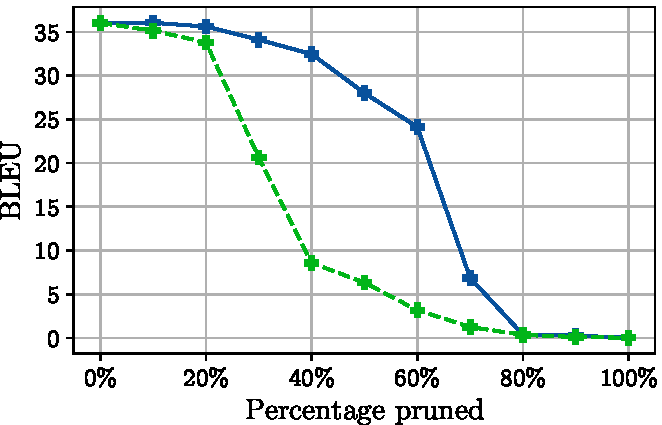
\includegraphics[width=\textwidth]{img/pruning_wmt.pdf}
\caption{\label{fig:incremental_pruning_wmt} Evolution of BLEU score on \texttt{newstest2013} when heads are pruned from \tfwmt{}.}
\end{subfigure}
~
\begin{subfigure}[t]{0.48\textwidth}
\centering
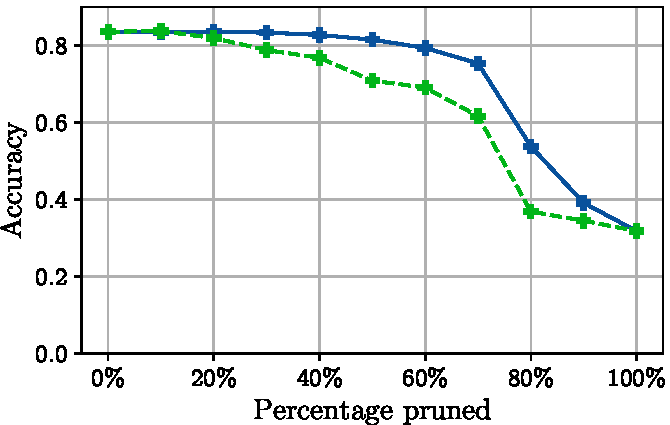
\includegraphics[width=\textwidth]{img/pruning_bert.pdf}
\caption{\label{fig:incremental_pruning_bert} Evolution of accuracy on the MultiNLI-matched validation set when heads are pruned from \bertmnli{}.}
\end{subfigure}
\caption{Evolution of accuracy by number of heads pruned according to $I_h$ (solid blue) and individual oracle performance difference (dashed green).}
\end{figure*}

% \paul{TODO: comment on results. Essentially we can prune a lot but not go down to one attention head per layer}. We add that we didn't re-train the pruned model, a process often used in the pruning literature \cite{} and susceptible to allow even more extreme sparsity.

We observe that this approach allows us to prune up to $20\%$ and $40\%$ of heads from \tfwmt{} and \bertmnli{} (respectively), without incurring any noticeable negative impact. Performance drops sharply when pruning further, meaning that neither model can be reduced to a purely single-head attention model without retraining or incurring substantial losses to performance. We refer to Appendix \ref{sec:additional_pruning} for experiments on four additional datasets.


\subsection{Effect of Pruning on Efficiency}

Beyond the downstream task performance, there are intrinsic advantages to pruning heads. First, each head represents a non-negligible proportion of the total parameters in each attention layer ($6.25\%$ for \tfwmt{}, $\approx 8.34\%$ for \bertmnli{}), and thus of the total model (roughly speaking, in both our models, approximately one third of the total number of parameters is devoted to \ac{mha} across all layers).\footnote{Slightly more in \tfwmt{} because of the Enc-Dec attention.} This is appealing in the context of deploying models in memory-constrained settings.

% \begin{table*}[!h]
% \centering
% \begin{tabular}{c|ccc}
%  & single example & batched (32)\\
% \hline\hline
% Original model & 16.55 & 126.57 \\\hline
% \multirow{2}{*}{-50\% heads}  & 29.95 & 127.03 \\
%   & (+80.98\%) & (+0.37\%) \\
% \hline
% \end{tabular}
% \caption{\label{tab:pruning_speedup} Average inference speed of BERT on the MNLI-matched validation set (in examples per second). The speedup relative to the original model is indicated in parentheses.}
% \end{table*}


\begin{table*}[!h]
% \begin{table}[!h]
\centering
{\small
\begin{tabular}{c|cccc}
%  & single example & batched (32)\\
Batch size & 1 & 4 & 16 & 64 \\
\hline\hline
Original & $17.0\pm 0.3$ & $67.3\pm 1.3$ & $114.0\pm 3.6$ & $124.7\pm 2.9$ \\
Pruned (50\%) & $17.3\pm 0.6$ & $69.1\pm 1.3$ & $134.0\pm 3.6$ & $146.6\pm 3.4$ \\
 & (+1.9\%) & (+2.7\%) & (+17.5\%) & (+17.5\%) \\
\hline
\end{tabular}
\caption{\label{tab:pruning_speedup}{\footnotesize Average inference speed of BERT on the MNLI-matched validation set in examples per second ($\pm$ standard deviation). The speedup relative to the original model is indicated in parentheses.}}
}
\end{table*}

Moreover, we find that actually pruning the heads (and not just masking) results in an appreciable increase in inference speed. Table \ref{tab:pruning_speedup} reports the number of examples per second processed by \bertmnli{}, before and after pruning 50\% of all attention heads. Experiments were conducted on two different machines, both equipped with GeForce GTX 1080Ti GPUs. Each experiment is repeated 3 times on each machine (for a total of 6 datapoints for each setting).
We find that pruning half of the model's heads speeds up inference by up to $\approx17.5\%$ for higher batch sizes (this difference vanishes for smaller batch sizes).


% and neither model can be completely reduced to single-head attention, this still represents a significant reduction in the number of parameters, with potential benefits in terms of memory and time consumption.

% \omer{placing here temporarily}
% Not only is single-head attention less expressive than multi-head attention, but as a by-product this reduces the number of parameters in the attention layer by $93.75\%$ \gn{This last sentence seems out of place here. Maybe it would fit better in Section \ref{sec:pruning}}.





% \subsection{Is Multi-headedness Equally Important in Different Parts of the Model?}

